


\newarray\states
\readarray{states}{1111 & 1110 & 1101 & 1100 & 1011 & 1010 & 1001 & 1000 & 0111 & 0110 & 0101 & 0100 & 0011 & 0010 & 0001 & 0000}


\noindent\makebox[\textwidth]{%
    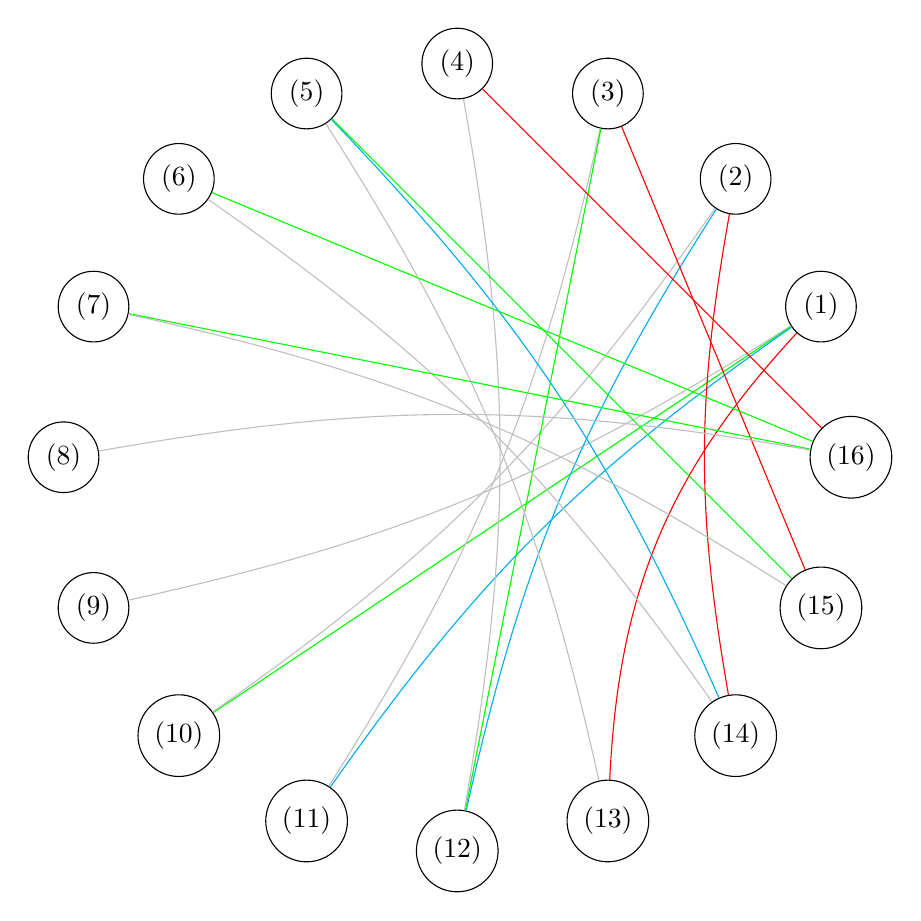
\begin{tikzpicture}[block/.style={circle,thick}]

        \foreach \a in {1,...,16}{
            \draw (\a*360/16: 5cm) node[shape=circle,draw=black](\a){\states(\a)};
        }

    \fill[fill=red] (1);
    \draw ->(1);
    \draw (1) to[bend left=10] (9)  [draw=lightgray];
    \draw (1) to (10) [draw=green];
    \draw (1) to[bend right=10] (11) [draw=cyan];
    \draw (1) to[bend right=20] (13) [draw=red];

    \draw (2) to[bend left=10] (10) [draw=lightgray];
    \draw (2) to[bend right=10] (12) [draw=cyan];
    \draw (2) to[bend right=10] (14) [draw=red];

    \draw (3) to[bend left=10] (11) [draw=lightgray];
    \draw (3) to (12) [draw=green];
    \draw (3) to (15) [draw=red];

    \draw (4) to[bend left=10] (12) [draw=lightgray];
    \draw (4) to (16) [draw=red];

    \draw (5) to[bend left=10] (13) [draw=lightgray];
    \draw (5) to[bend left=10] (14) [draw=cyan];
    \draw (5) to (15) [draw=green];

    \draw (6) to[bend left=10] (14) [draw=lightgray];
    \draw (6) to (16) [draw=green];

    \draw (7) to (16) [draw=green];
    \draw (7) to[bend left=10] (15) [draw=lightgray];

    \draw (8) to[bend left=10] (16) [draw=lightgray];



    \end{tikzpicture}
}
